\documentclass{standalone}
\usepackage{tikz}
\usepackage{ctex,siunitx}
\setCJKmainfont{Noto Serif CJK SC}
\usepackage{tkz-euclide}
\usepackage{amsmath}
\usepackage{wasysym}
\usetikzlibrary{patterns, calc}
\usetikzlibrary {decorations.pathmorphing, decorations.pathreplacing, decorations.shapes,}
\begin{document}
\small
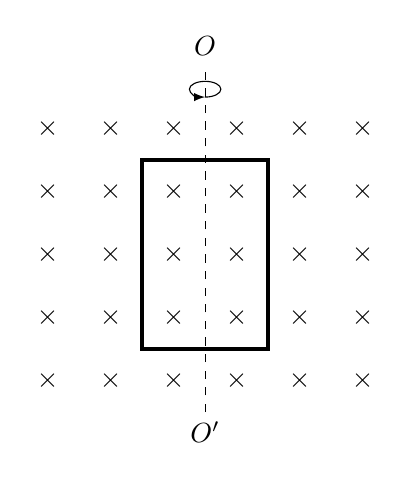
\begin{tikzpicture}[>=latex,scale=0.8]
  % \useasboundingbox(0.9,0)rectangle(5.1,5);
  \foreach \x in {-3,-2,...,2}
  \foreach \y in {-2,...,2}
  {
      \node at (\x,\y){$\times$};
  }
  \draw [dashed](-.5,-2.5)node[below]{$O'$}--(-.5,3)node[above]{$O$};
  \draw[very thick] (-1.5,-1.5) rectangle (.5,1.5);
  \draw[->] (-.5, 2.5) arc [start angle=-90, end angle=270, x radius=.25,y radius=.125];
\end{tikzpicture}
\end{document}